%%%%%%%%%%%%%%%%%%%%%%%%%%%%%%%%%%%%%%%%%
% Journal Article
% LaTeX Template
% Version 1.3 (9/9/13)
%
% This template has been downloaded from:
% http://www.LaTeXTemplates.com
%
% Original author:
% Frits Wenneker (http://www.howtotex.com)
%
% License:
% CC BY-NC-SA 3.0 (http://creativecommons.org/licenses/by-nc-sa/3.0/)
%
%%%%%%%%%%%%%%%%%%%%%%%%%%%%%%%%%%%%%%%%%

%----------------------------------------------------------------------------------------
%	PACKAGES AND OTHER DOCUMENT CONFIGURATIONS
%----------------------------------------------------------------------------------------

\documentclass[twoside]{article}

\usepackage{lipsum} % Package to generate dummy text throughout this template

\usepackage[sc]{mathpazo} % Use the Palatino font
\usepackage[T1]{fontenc} % Use 8-bit encoding that has 256 glyphs
\linespread{1.05} % Line spacing - Palatino needs more space between lines
\usepackage{microtype} % Slightly tweak font spacing for aesthetics

\usepackage[hmarginratio=1:1,top=32mm,columnsep=20pt]{geometry} % Document margins
\usepackage{multicol} % Used for the two-column layout of the document
\usepackage[hang,small,labelfont=bf,up,textfont=it,up]{caption} % Custom captions under/above floats in tables or figures
\usepackage{booktabs} % Horizontal rules in tables
\usepackage{float} % Required for tables and figures in the multi-column environment - they need to be placed in specific locations with the [H] (e.g. \begin{table}[H])
\usepackage{hyperref} % For hyperlinks in the PDF

\usepackage{lettrine} % The lettrine is the first enlarged letter at the beginning of the text
\usepackage{paralist} % Used for the compactitem environment which makes bullet points with less space between them
\usepackage{graphicx} % Used for including images

\usepackage{abstract} % Allows abstract customization
\renewcommand{\abstractnamefont}{\normalfont\bfseries} % Set the "Abstract" text to bold
\renewcommand{\abstracttextfont}{\normalfont\small\itshape} % Set the abstract itself to small italic text

\usepackage{titlesec} % Allows customization of titles
\renewcommand\thesection{\Roman{section}} % Roman numerals for the sections
\renewcommand\thesubsection{\Roman{subsection}} % Roman numerals for subsections
\titleformat{\section}[block]{\large\scshape\centering}{\thesection.}{1em}{} % Change the look of the section titles
\titleformat{\subsection}[block]{\large}{\thesubsection.}{1em}{} % Change the look of the section titles

\usepackage{fancyhdr} % Headers and footers
\pagestyle{fancy} % All pages have headers and footers
\fancyhead{} % Blank out the default header
\fancyfoot{} % Blank out the default footer
\fancyhead[C]{Boulder Flood Impacts Pre-flood and Post-flood - 2013 $\bullet$ March 2015 $\bullet$ No. 1} % Custom header text
\fancyfoot[RO,LE]{\thepage} % Custom footer text

%----------------------------------------------------------------------------------------
%	TITLE SECTION
%----------------------------------------------------------------------------------------

\title{\vspace{-15mm}\fontsize{24pt}{10pt}\selectfont\textbf{Boulder Flood Impacts Pre-flood and Post-flood - 2013}} % Article title

\author{
\large
\textsc{John Raesly}\thanks{\url{http://jraesly.me}}\\[2mm] % Your name
\normalsize University of Colorado - Boulder \\ % Your institution
\normalsize \href{mailto:john.raesly@gmail.com}{john.raesly@gmail.com} % Your email address
\vspace{-3mm}
}
\date{3/29/2015}

%----------------------------------------------------------------------------------------

\begin{document}

\maketitle % Insert title

\thispagestyle{fancy} % All pages have headers and footers

%----------------------------------------------------------------------------------------
%	ABSTRACT
%----------------------------------------------------------------------------------------

\begin{abstract}

The 2013 flood in Boulder, called the 100 year flood, was a natural disaster for the century in Boulder. The floods' power changed much of the ecosystem that surrounds Boulder, CO. The purpose of this project is to examine the 2013 flood in Boulder, CO and its impacts on the river morphology of the creeks and rivers surrounding Boulder, CO and the change in land cover that occurred. Direct correlations between the rivers and the amount of rainfall in those areas feeding into the rivers are of particular interest. This study will investigate how river morphology has changed from pre to post flood? What is the correlation between rainfall amounts and the post-flood stream channel? QGIS will be utilized to perform file conversions and other usable formats for Grass GIS. Then Grass GIS will be used to integrate an analysis method for the raster data and dissolve it as necessary. Previous techniques from other flood studies that have shown to be effective will be analyzed. Sources will include the Boulder Open GIS, which has some from the NOAA Disaster Data to analyze similar conditions (rainfall amount). This study will focus on Boulder County in Colorado. 51.6\% of the post-flood stream channel is additional length compared to the pre-flood stream channel. Using Shreve's Stream Ordering method there was a staggering difference between the stream order of the pre-flood and post-flood. 

\end{abstract}

%----------------------------------------------------------------------------------------
%	ARTICLE CONTENTS
%----------------------------------------------------------------------------------------

\begin{multicols}{2} % Two-column layout throughout the main article text

\section{Introduction}

\lettrine[nindent=0em,lines=3]{U}nderstanding the river morphology for the Boulder 2013 Flood is important for assesing the floodplains that are at the top concern if such an event were to happen again. The 2013 flood in Boulder was a natural disaster that could be cause for concern. The flood changed the stream channel within Boulder County, CO. The flood caused a total of 3 fatalities during its 8 day rain period. 306 people are still reported as missing (as of September 19th 2013). The flood had affected an area estimated to be 4,500 square miles --- roughly the size of Jamaica. 12,118 people were under mandatory evacuation orders and 1,000 people had to be airlifted to safety from remote locations, the largest airlift resuce operation in USA since Katrina. 1,502 homes destroyed, 17,494 homes damaged (Colorado Office of Emergency Management estimates) and 30 (state-maintained) bridges destroyed, 20 (state-maintaned) bridges damaged (according to Colorado Department of Transportation). \cite{facts} This study focuses specifically on Boulder County. In this study, the 2013 flood in Boulder, CO is examined and its impacts on the river morphology of the creeks and rivers surrounding Boulder, CO and the change in land cover that occurred. Direct correlations between the rivers the amount of rainfall in those areas feeding into the rivers are of interest. In particular, this study will investigate how river morphology has changed from pre to post flood? What is the correlation between rainfall amounts and the post-flood stream channel?
%------------------------------------------------

\section{Data}
The data for this study was gathered from the Boulder Open GIS (Geographic Information Systems) on the Boulder County government website. The data gathered from Boulder Open GIS is in State Plan Coordinate System explicitly in Feet. This data is free to use and be distrubuted. Some of this data is sourced from a make up of NOAA's Disaster Data. NOAA (National Oceanic and Atmospheric Administration) is an American scientific agency within the United States Department of Commerce focused on the conditions of the oceans and the atmosphere. \cite{NOAA} The rainfall amounts on the Boulder Open GIS website were a compilation of all the days added into one dataset. 


\section{Methods}

Several measures were developed to assess the stream channel - pre flood against the stream channel - post flood shapefiles.
\begin{compactitem}
\item Clip the shapefiles
\item Find the difference in the shapefiles
\item Assign rainfall minimum and maximum attribute for Boulder County
\item Assign general rainfall minimum and maximum to separated areas
\item Correlate the rainfall amounts against the post-flood stream channel
\item Stream Ordering Using the Shreve Method

\end{compactitem}

\subsection{Clip the Shapefiles}
QGIS was used for most operations during this research. Using the built-in function, Clip was able to show the similarities in both of the shapefiles. It created a new shape based on the area of the input layer that is overlapped by the clipping layer. The attributes of the chosen layer only were copied to the new feature with the new information, of which parts stayed the same. It was then useful to examine the portion that did not change. Notably, only a small portion of the stream channel did not change.


\subsection{Find the Difference in Shapefiles}
The difference function in QGIS was then used to determine the difference in the two shapefiles being examined. Both of the shapefiles had the same attributes which made it simpler to compare and contrast. The difference function created a new feature based on the area of the input layer that was not overlapped by the clipping layer.


\subsection{Assign Rainfall Attribute for Boulder County}

\begin{figure*} % figure* spans two columns, figure is just one column
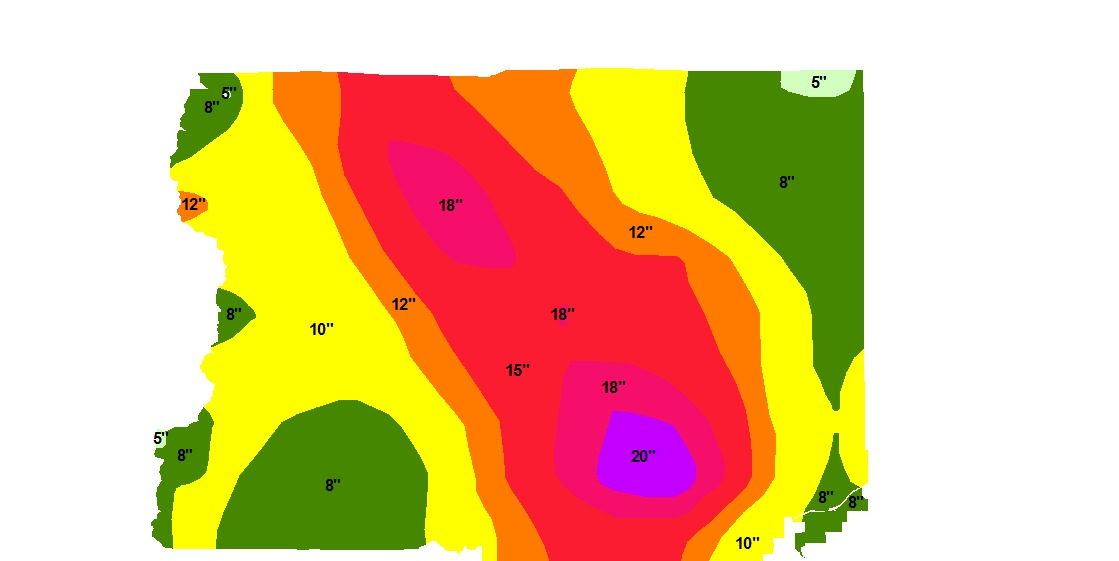
\includegraphics[width=2\columnwidth]{project.jpg}
\caption{Rainfall Distribution\label{fig:sloth}}
\end{figure*}


The purpose of this part was to assign a general legend for each area that fell into similar rainfall mininum and maximum ranges. The numbers can be viewed in figure 1. It was based upon finding a general rule for each set of values for the designated areas. The shapefile from Boulder Open GIS about the rainfall amounts had an attribute table similar to Table 1. Excluded in the table below was the Shape\_area and Shape\_len which delineated the ObjectID's location. As can be seen in Table 1, the locations had fairly similar results, which made the creation of the Figure 1 easy to produce.


\begin{table}[H]
\caption{Rainfall Amount Attribute Table}
\centering
\begin{tabular}{llr}
\cmidrule(r){1-3}
ObjectID & RainfallMi & RainfallMa \\
\midrule
1 & $8$ & $10$  \\
2 & $6$ & $8$ \\
3 & $6$ & $8$ \\
4 & $8$ & $10$ \\
5 & $10$ & $12$ \\
6 & $12$ & $15$ \\
7 & $10$ & $12$ \\
8 & $6$ & $8$ \\
9 & $10$ & $12$ \\
10 & $6$ & $8$ \\
11 & $6$ & $8$ \\
12 & $6$ & $8$ \\
13 & $15$ & $18$ \\
14 & $15$ & $18$ \\
15 & $15$ & $18$ \\
16 & $18$ & $20$ \\
17 & $4$ & $5$ \\
18 & $4$ & $5$ \\
19 & $4$ & $5$ \\
20 & $6$ & $8$ \\
\bottomrule
\end{tabular}
\end{table}


\subsection{Correlate Rainfall and Post-flood River Morphology}

\begin{figure}[H] % figure* spans two columns, figure is just one column
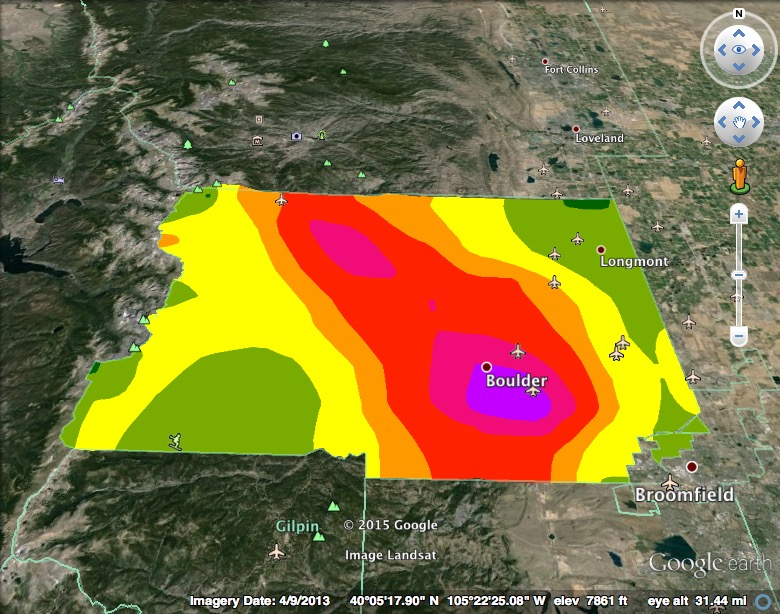
\includegraphics[width=1\columnwidth]{earth.jpg}
\caption{Rainfall Distribution over Boulder County\label{fig:earth}}
\end{figure} 

The correlation was created by implementing Spatial Autocorrelation within QGIS. Spatial Autocorrelation is a measure of the degree to which a set of spatial features and their associated data values tend to be clustered together in space (positive spatial autocorrelation) or dispersed (negative spatial autocorrelation). \cite{spatial} It was also easily viewed by overlapping the rainfall data with the post-flood stream channel shapefile, which can be viewed in Figure 4. In regards to the areas that acquired a larger amount of rainfall, it is evident that more stream channels came to be after.

\begin{figure}[H] % figure* spans two columns, figure is just one column
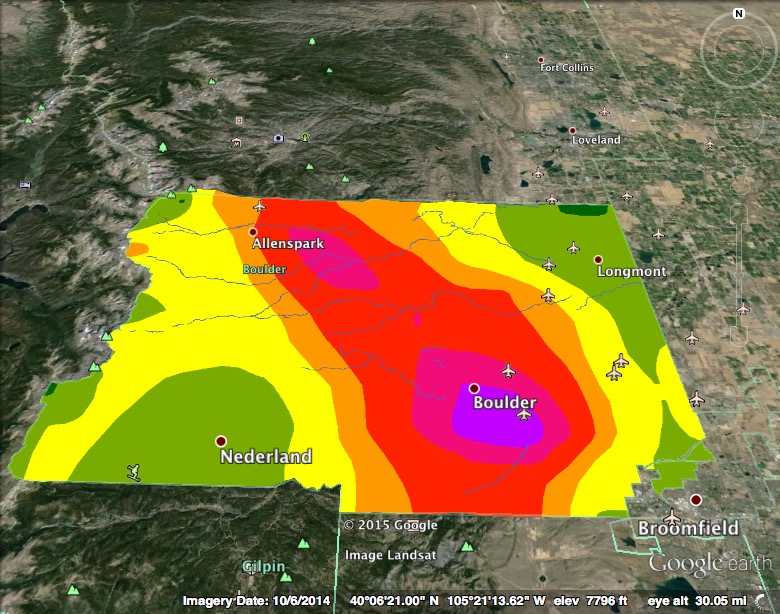
\includegraphics[width=1\columnwidth]{preflood.jpg}
\caption{Pre-Flood Stream Channel and Rainfall Distribution\label{fig:preflood}}
\end{figure} 

\begin{figure}[H] % figure* spans two columns, figure is just one column
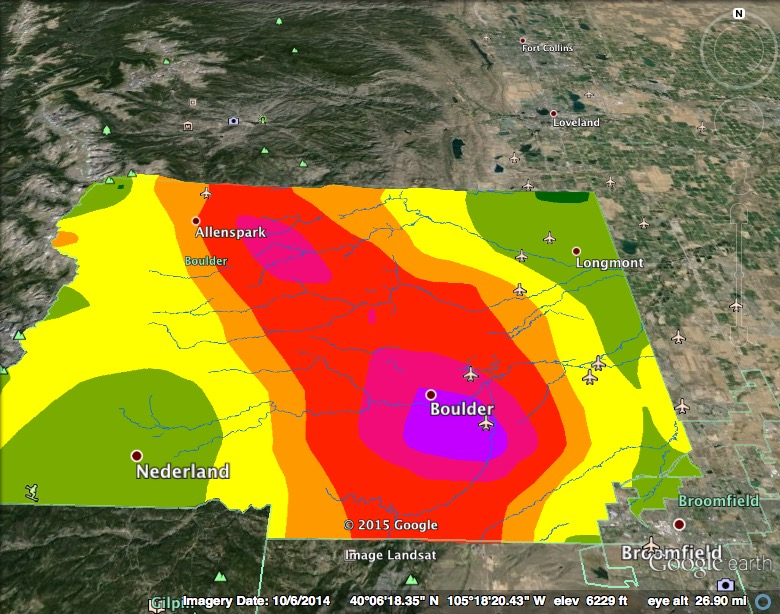
\includegraphics[width=1\columnwidth]{postflood.jpg}
\caption{Post-Flood Stream Channel and Rainfall Distribution\label{fig:postflood}}
\end{figure}

\subsection{Stream Ordering using Shreve}
The most common method for determining is the Strahler Method. The disadvantage of Strahler's method is the lack of distinguishing a main channel which may interfere with the analytical process in highly elongated catchments. \cite{Strahler} Shreve's method was used in this study to determine the stream order. Shreve's method is less strict in approaching its stream ordering. This was a stretch in the study because of the difficulty to reproduce the vectors as raster data and in order to find the stream order the input file has to be in a raster format. There is a method for vectors using v.strahler in Grass GIS, but it is currently experimental and requires a DEM (Digital Elevation Model) which is a 3D representation of a terrain's surface. Finding a useful (and free) DEM of Boulder County proved to be exhaustive. Using gdal\_rasterize produced an image with just a bunch of points along the path that used to be the stream channel. A workaround though was discovered by extracting the nodes in the vector. After the nodes were extracted, it was possible to rasterize the vector using gdal\_rasterize. This made a colorful picture of the stream channels. One of the next requirements for finding stream order was having the Flow Direction raster. The Stream Order uses the raster input of the node raster against the flow direction raster. 

\begin{table}[H]
\caption{Shreve Pre Flood Stream Order}
\centering
\begin{tabular}{llr}
\cmidrule(r){1-2}
Value & Count \\
\midrule
1 & $2038$ \\
2 & $11$ \\
3 & $6$ \\
4 & $1$ \\
\bottomrule
\end{tabular}
\end{table}



\begin{table}[H]
\caption{Shreve Post Flood Stream Order}
\centering
\begin{tabular}{llr}
\cmidrule(r){1-2}
Value & Count \\
\midrule
1 & $3539$ \\
2 & $65$ \\
3 & $26$ \\
4 & $4$ \\
5 & $1$ \\
\bottomrule
\end{tabular}
\end{table}


%------------------------------------------------
\section{Results}
 
Only 48.4\% of the post-flood stream channel stayed consistent with the pre-flood stream channel during this disaster. In contrast, 51.6\% of the stream length was newly accounted for after the 2013 Boulder Flood. The stream area had very similar findings for its catagory.The stream area found the same way as the stream length by summing all of the stream areas attributes. Discovered was a 49.4\% increase in the stream area. By using this information we can conclude that there was a 1\% increase in width. The average pre-flood width was 10.750317413 feet while the average post-flood width was 11.211486364 feet. 
\begin{figure*} % figure* spans two columns, figure is just one column
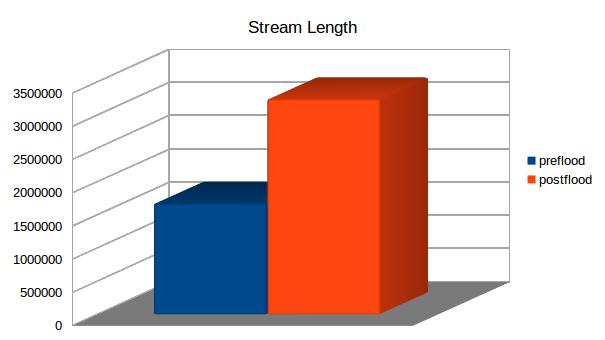
\includegraphics[width=2\columnwidth, scale=2]{prevspostlength.jpg}
\caption{Pre Flood Stream Length and Post Flood Stream Length\label{fig:length}}
\end{figure*}

The mass of the findings concluded that most of the now stream channel was newly created. The post-flood stream channel is mostly represented by the rainfall that happened during the flood. Where there was less rain, most of those channels have dissapeared and dispersed into the areas where there was the most rainfall. There was very little stream channel in Boulder, CO pre-flood, but now there are many new streams that have been created because of this flood and it mostly amounts to the mass rainfall that was recorded in the Southern part of the county. In Tables 2 and 3, the stream order for pre flood and post flood are calculated. The way to interpret this data is from bottom to top. Value 4 of Table 2 and value 5 of Table 3 are the stems of the stream channel. Value 1 for each table are the parts of the stream without any branches. The post flood stream order has one more value in its stem which concludes that the stream channel is much more comprehensive than it was before the flood. The amount of ending branches is much larger in the post flood stream order than pre flood. The results in the tables can be misleading when comparing it to figures 3 and 4 because although in the figures it may not look like there are over 3,000 branches in Figure 4. In the vectors used for Figures 3 and 4, there are hidden features that cannot be shown. These features were extracted using the method described in Section Five of Methods. If zoomed in many layers, it is possible to see the disconnections that are within the stream channel. These disconnects would be considered their own stream and thus be determined a value of 1. In Figure 5, a bar graph was created by summing the stream lengths for pre flood and post flood. 
\newline
\begin{figure*} % figure* spans two columns, figure is just one column
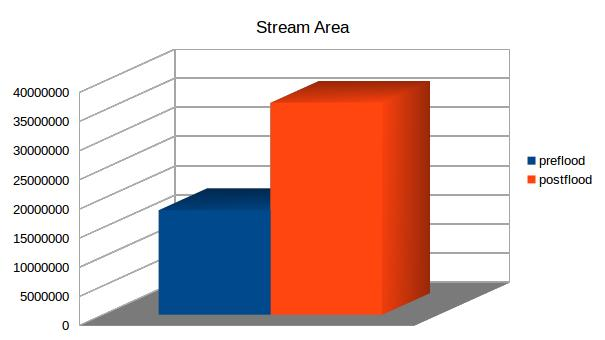
\includegraphics[width=2\columnwidth, scale=2]{prevspostarea.jpg}
\caption{Pre Flood Stream Length and Post Flood Stream Area\label{fig:length}}
\end{figure*}


%------------------------------------------------

\section{Discussion}

The entirety of this disaster created many new stream channels throughout Boulder County. Whereas most of the stream channel occured in the Northwestern part of the county it is now distributed evenly throughout the county with more of it leaning towards the eastern border. Large amounts of rainfall can be extremely effective in rerouting a whole river system. This causes many unknown side effects. There could be a loss of habitat in the area that for so long had relied on the river system, but the newly created streams could thrive and welcome all new sorts of habitat. This does mess up the ecological balance that nature depends on.


\section{Limitations}

Since there was not a lot of time alloted for this study, there were some limitations. The nature of the vectors provided by Boulder Open GIS did not include any information about the river density which was a subject of interest. It would have been beneficial to look at multiple other sources for data to see if there were any conflicting results. As most weather companies have their own rain catchers', some of the resulting rainfall data could have changed from a day to day basis.  As there are now many reasons to attribute to habitat loss, i.e. global warming, the main focus should be upon the species that whole heartedly relied upon the previous river system. Another focus of study should be if there are new disasters that were previously averted because of the river morphology. One of the disasters could be the snow melt and the floodplains. For instance, does the new stream channel cause concern for residents situated around these floodplains that were previously unaffected?

\section{Conclusion}
While the news may tell you the certain aspects of the Boulder 2013 Flood, they are not able to show the affects it has had on our community within Boulder County. It is apparent after careful research, that the Boulder 2013 Flood, was a natural disaster, which has changed the river morphology of the creeks and surrounding rivers of Boulder County. The stream channel prior to the flood (Figure 3) is minimal compared to the significant increase after the flood, as seen in Figure 4. This shows a direct correlation between the rivers and the amount of rainfall feeding into the rivers. Not only did the number of rivers multiply, but also the length of the existing rivers and streams increased. The conclusions derived from this research could be beneficial to other GIScientists who will further study the now unknown effects this will have on Boulder County's wildlife. It is too soon to know the ecological impact of such a flood, however, it is important to recognize the change in the river and stream morphology as an indicator of other changes happening within the surrounding ecosystem. Although it is not an unknown topic, using the techniques in river morphometry have proved themselves beneficial for this study and hopefully future studies will use these techniques for describing the river morphology in their study.



%----------------------------------------------------------------------------------------

%----------------------------------------------------------------------------------------
%	REFERENCE LIST
%----------------------------------------------------------------------------------------

\begin{thebibliography}{100} % Bibliography - this is intentionally simple in this template

\bibitem{facts}
\newblock "Colorado Flood Facts and Figures --- FloodList." FloodList. September 19, 2013. Accessed May 3, 2015. \url{http://floodlist.com/america/usa/colorado-flood-facts-figures}.

\bibitem{NOAA}
\newblock "National Oceanic and Atmospheric Administration." Wikipedia. Accessed May 3, 2015. \url{http://en.wikipedia.org/wiki/National_Oceanic_and_Atmospheric_Administration}.

\bibitem{spatial}
\newblock "GIS Dictionary." Spatial Autocorrelation. Accessed May 4, 2015. \url{http://support.esri.com/en/knowledgebase/GISDictionary/term/spatial\%20autocorrelation} .


\bibitem{Strahler}
\newblock Jasiewicz, Jarek. "GRASS GIS Manual: R.stream.order." GRASS GIS Manual: R.stream.order. December 27, 2014. Accessed May 4, 2015. \url{http://grass.osgeo.org/grass70/manuals/addons/r.stream.order.html}.

\end{thebibliography}

%----------------------------------------------------------------------------------------


\end{multicols}

\end{document}
